\documentclass[../../main.tex]{subfiles}
\graphicspath{{../../image/}{../../figure/}}
\begin{document}

\section{耦合流}\label{section:ch18-耦合流}

本章将讨论训练非线性潜变量模型的 $4$ 种方法中的第 $2$ 种方法（参见 16.4.4 小节），它通过限制神经网络模型的形式，在确保能够从训练好的模型中易于采样的前提下，无须近似即可计算似然函数。假设我们定义了一个分布 $p_z(z)$（有时也称\textbf{基础分布}（base distribution）），这个分布定义在潜变量 $z$ 上，以及一个由深度神经网络给出的非线性函数 $x=f(z,w)$，该函数要将潜空间转换成数据空间。假设 $p_z(z)$ 是一个简单的分布，比如高斯分布，那么从这样的模型中抽样就很容易，因为每一个潜样本 $z\sim p_z(z)$ 只需要通过神经网络就可以生成对应的数据样本 $x=f(z,w)$。

为了计算这个模型的似然函数，我们需要知道数据空间分布，而它依赖于神经网络函数的逆函数，记为 $z=g(x,w)$，并且满足 $z=g(f(z,w),w)$。这要求对于每一个 $w$ 值，函数 $f(z,w)$ 和 $g(x,w)$ 都是可逆的，也称为\textbf{双射}（bijective），即每个 $x$ 值都对应唯一的 $z$ 值，反之亦然。然后我们可以使用变量变换公式来计算数据密度（参见 2.4 节）：
\begin{align}
p_x(x\mid w)=p_z\big(g(x,w)\big)\,|\det J(x)|
\label{align:ch18-change-var}
\end{align}
其中 $J(x)$ 是偏导数的雅可比矩阵，其元素由 $J_{ij}=\partial z_i/\partial x_j$ 给出。式~\eqref{align:ch18-change-var} 中的 $|\cdot|$ 表示模或绝对值。尽管确定性映射意味着任何给定的数据值 $x$ 都对应一个唯一的 $z$ 值，$z$ 值因此不再不确定，但我们仍继续将 $z$ 称为``潜变量''。

考虑一个训练集 $\mathcal{D}=\{x_1,\cdots,x_N\}$，它由独立数据点组成，根据式~\eqref{align:ch18-change-var} 得到的对数似然函数为
\begin{align}
\ln p(\mathcal{D}\mid w)=\sum_{n=1}^{N}\ln p_z\big(g(x_n,w)\big)+\sum_{n=1}^{N}\ln|\det J(x_n)|
\label{align:ch18-loglik}
\end{align}
要求可逆映射的一个结果是潜空间的维度必须与数据空间的维度相同，这可能导致像图像这样的高维数据会需要很大的模型。另外，评估 $D\times D$ 矩阵的行列式的成本通常是 $\mathcal{O}(D^3)$，所以我们需要对模型施加一些额外的限制，以便更高效地计算雅可比行列式。

我们的目标是使用似然函数来训练神经网络。为了能够建模各种各样的分布，我们希望转换函数 $x=f(z,w)$ 高度灵活，因而使用了深度神经网络架构。如果能够保证网络的每一层都是可逆的，那么整个函数就是可逆的（见习题 18.2）。考虑三个连续的转换，其中的每个转换对应于一个层，形式如下：
\begin{align}
x=f_1(f_2(f_3(z)))
\label{align:ch18-three-layers}
\end{align}
逆函数为
\begin{align}
z=g_3(g_2(g_1(x)))
\label{align:ch18-inv-layers}
\end{align}
其中 $g_1,g_2,g_3$ 分别是 $f_1,f_2,f_3$ 的逆函数。此外，可以使用微积分链式规则计算每个单独层的雅可比行列式，这种分层结构的雅可比行列式也很容易得到。式~\eqref{align:ch18-inv-layers} 的右侧为三个矩阵的乘积，而乘积的行列式是行列式的乘积。因此，整体雅可比矩阵的对数行列式将是每层对应对数行列式之和（参见附录~A）。

这种对灵活分布进行建模的方法称为\textbf{标准化流}（normalizing flow），因为通过一系列映射来转换概率分布的过程在某种程度上类似于流体的流动。此外，逆映射的效果是将复杂的数据分布转换成标准化形式，通常是高斯分布。我们将讨论实践中经常使用的两个主要类型的标准化流的核心概念：耦合流（coupling flow）和自回归流（autoregressive flow）。此外，我们还将介绍使用神经微分方程定义可逆映射的方法，并引入连续流（continuous flow）这一概念。

\subsection{实值 NVP}\label{subsection:ch18-realnvp}

我们的目标是设计一个单一的可逆函数层，这样就可以将许多这样的层组合在一起，从而定义一类高度灵活的可逆函数。首先考虑以下形式的线性变换：
\begin{align}
x=az+b
\label{align:ch18-linear}
\end{align}
这个变换很容易求逆，得到
\begin{align}
z=(x-b)/a
\label{align:ch18-linear-inv}
\end{align}
然而，线性变换在组合下是封闭的，这意味着一系列线性变换等同于一个整体的线性变换（见习题 3.6）。因为，高斯分布的线性变换结果还是高斯分布。所以即使我们有许多这样的线性变换``层''，我们也只能得到一个高斯分布。问题在于我们能否保持线性变换的可逆性，同时允许额外的灵活性，从而使得最终结果可以是非高斯分布。

解决这个问题的一种方法是使用一个叫作\textbf{实值 NVP}（real-valued non-volume-preserving, RealNVP）（Dinh, Krueger, and Bengio, 2014; Dinh, Sohl-Dickstein, and Bengio, 2016）的标准化流模型。这里的 NVP 代表非体积保持（non-volume-preserving）。其思想是将潜变量向量 $z$ 划分为两部分，$z=(z_A,z_B)$，如果 $z$ 的维度为 $D$ 且 $z_A$ 的维度为 $d$，则 $z_B$ 的维度为 $D-d$。我们可以类似地划分输出向量，$x=(x_A,x_B)$，其中 $x_A$ 的维度为 $d$，$x_B$ 的维度为 $D-d$。对于输出向量的第一部分，我们简单地复制输入
\begin{align}
x_A=z_A
\label{align:ch18-xa}
\end{align}
输出向量的第二部分经历了一个线性变换，但这个线性变换中的系数由 $z_A$ 的非线性函数给出：
\begin{align}
x_B=\exp\big(s(z_A,w)\big)\odot z_B+b(z_A,w)
\label{align:ch18-coupling}
\end{align}
其中 $s(z_A,w)$ 和 $b(z_A,w)$ 是神经网络的实值输出，指数函数确保了乘法项是非负的。这里的 $\odot$ 表示哈达玛积（Hadamard product），即对两个向量进行逐元素相乘。在式~\eqref{align:ch18-coupling} 中，指数也是逐元素计算的。

由于使用了神经网络函数，$x_B$ 的值可以是 $z_A$ 的一个非常灵活的函数。尽管如此，整体的变换仍然很容易逆推。给定 $x=(x_A,x_B)$ 的值，首先计算
\begin{align}
z_A=x_A
\label{align:ch18-za}
\end{align}
然后计算 $s(z_A,w)$ 和 $b(z_A,w)$，最后使用下式计算 $z_B$：
\begin{align}
z_B=\exp\big(-s(z_A,w)\big)\odot\big(x_B-b(z_A,w)\big)
\label{align:ch18-inv-coupling}
\end{align}

整体变换如图~\ref{fig:ch18-nvp-layer} 所示。注意，单个神经网络函数，如 $s(z_A,w)$ 和 $b(z_A,w)$，并不要求是可逆的。

\begin{figure}[htbp]
\centering
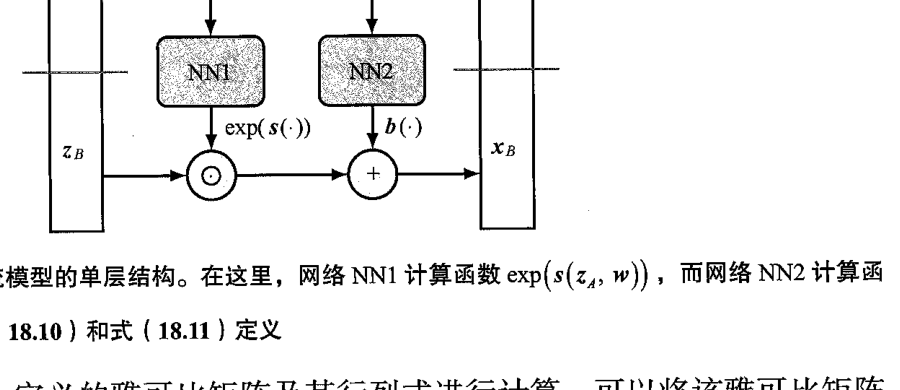
\includegraphics[width=0.75\textwidth]{ch18-fig498-nvp-layer.png}
\caption{实值 NVP 标准化流模型的单层结构。在这里，网络 NN1 计算函数 $\exp\{s(z_A,w)\}$，而网络 NN2 计算函数 $b(z_A,w)$。}
\label{fig:ch18-nvp-layer}
\end{figure}

考虑对式~\eqref{align:ch18-change-var} 定义的雅可比矩阵及其行列式进行计算。可以将该雅可比矩阵分成块，对应于 $z$ 和 $x$ 的划分，得到
\begin{align}
J=\begin{pmatrix}
\dfrac{\partial z_A}{\partial x_A} & \dfrac{\partial z_A}{\partial x_B}\\[4pt]
\dfrac{\partial z_B}{\partial x_A} & \dfrac{\partial z_B}{\partial x_B}
\end{pmatrix}
\label{align:ch18-block-jacobian}
\end{align}
其中，左上角的块对应于 $z_A$ 关于 $x_A$ 的导数，根据式~\eqref{align:ch18-za}，结果为 $d\times d$ 的单位矩阵。右上角的块对应于 $z_A$ 关于 $x_B$ 的导数，根据式~\eqref{align:ch18-za}，结果为 $0$。左下角的块对应于 $z_B$ 关于 $x_A$ 的导数，根据式~\eqref{align:ch18-inv-coupling}，这是关于神经网络函数的复杂表达式。最后，右下角的块对应于 $z_B$ 关于 $x_B$ 的导数，根据式~\eqref{align:ch18-inv-coupling}，这些导数由一个对角矩阵表示，其对角元素是 $\exp(-s(z_A,w))$。因此我们看到该雅可比矩阵是一个下三角块矩阵，其行列式只是沿主对角线元素的乘积，而不依赖于左下角的块中的复杂表达式。

因此，雅可比行列式可以简单地由 $\exp(s(z_A,w))$ 中元素的乘积给出。这种方法的一个明显局限是，$z_A$ 的值没有因变换而改变。这可以通过添加另一层来轻松解决，其中 $z_A$ 和 $z_B$ 的角色被颠倒过来，如图~\ref{fig:ch18-two-layer} 所示。这种双层结构可以重复多次，从而能构建一类非常灵活的生成式模型。

\begin{figure}[htbp]
\centering
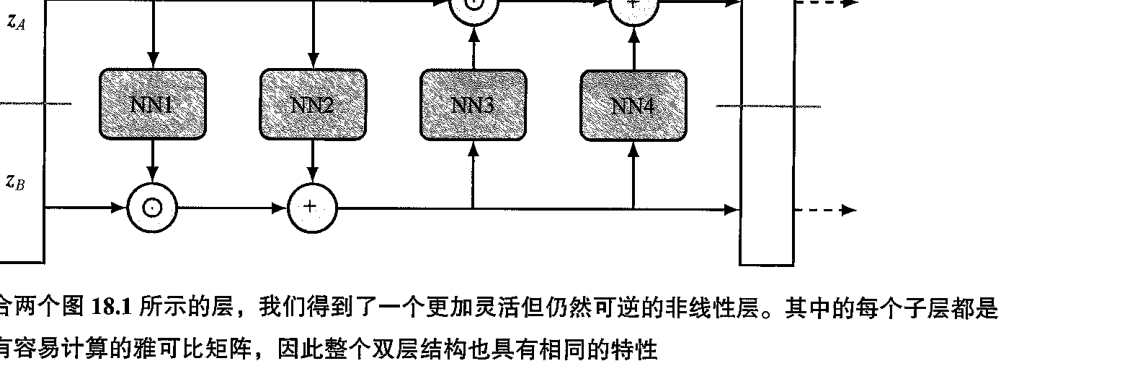
\includegraphics[width=0.85\textwidth]{ch18-fig499-two-layer.png}
\caption{通过组合两个图~\ref{fig:ch18-nvp-layer} 所示的层，我们得到了一个更加灵活但仍然可逆的非线性层。其中的每个子块都是可逆的，并且拥有容易计算的雅可比矩阵，因此整个双层结构也具有相同的特性。}
\label{fig:ch18-two-layer}
\end{figure}

实值 NVP 模型属于一类使用广泛的标准化流，称为\textbf{耦合流}（coupling flows）。在耦合流中，线性变换 [式~\eqref{align:ch18-coupling}] 被如下更一般的形式替换：
\begin{align}
x_B=h\big(z_B,g(z_A,w)\big)
\label{align:ch18-general-coupling}
\end{align}
其中 $h(z_B,g)$ 是 $z_B$ 的函数，对于任何给定的 $g$ 值，它都可以高效地逆推，称为\textbf{耦合函数}（coupling function）。$g(z_A,w)$ 称为\textbf{条件函数}（conditioner），通常用神经网络来表示。

整个训练过程包括创建数据点的一些小批量，在这些小批量中，每个数据点对对数似然函数的贡献可从式~\eqref{align:ch18-loglik} 中获得。对于形式为 $\mathcal{N}(z\mid 0,I)$ 的潜分布，对数密度就是 $-\|z\|^2/2$ 加一个加法常数。逆变换 $z=g(x)$ 可以使用一系列形式为式~\eqref{align:ch18-inv-coupling} 的逆变换计算得出。同样，雅可比行列式的对数由每层的对数行列式之和给出，其中的每一项本身就是形式为 $-s_i(x,w)$ 的项之和。

我们可以使用一个简单的数据集来说明实值 NVP 标准化流，这个数据集有时称为``双月''数据集，如图~\ref{fig:ch18-two-moons} 所示。在这里，一个二维高斯分布通过使用两个连续的层被转换成一个更复杂的分布，其中每一层都对输入数据的两个维度交替进行耦合变换。

\begin{figure}[htbp]
\centering
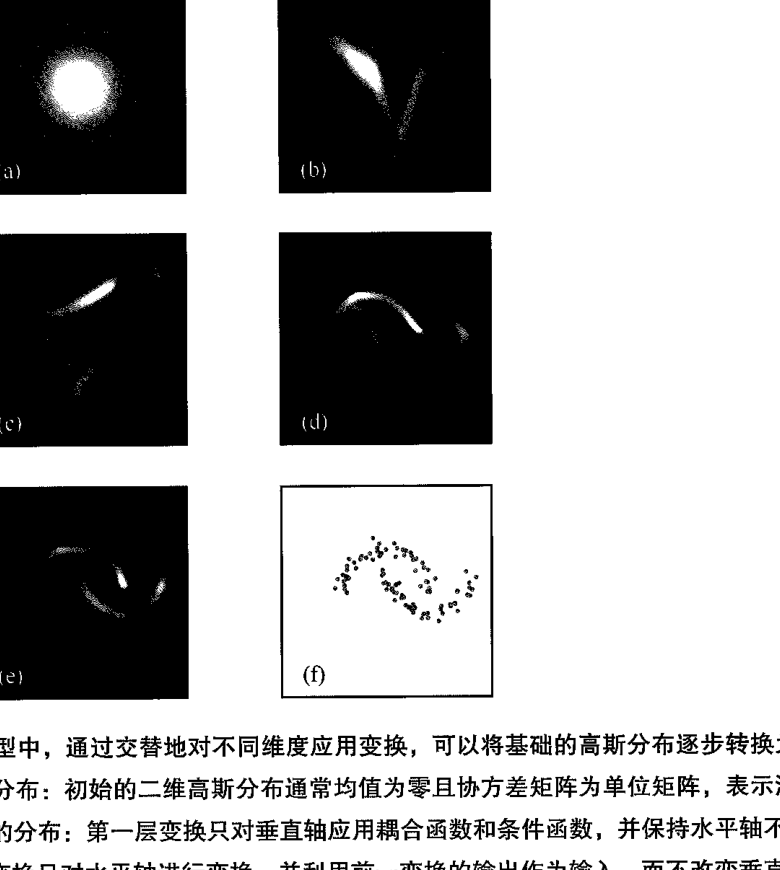
\includegraphics[width=0.9\textwidth]{ch18-fig500-two-moons.png}
\caption{在实值 NVP 标准化流模型中，通过交替地对不同维度应用变换，可以将基础的高斯分布逐步转换为更复杂的数据分布：(a) 基础的高斯分布；(b) 垂直轴变换后的分布；(c) 水平轴变换后的分布；(d) 第二次垂直轴变换后的分布；(e) 第二次水平轴变换后的分布；最终得到与训练集相匹配的复杂形状，即所谓的``双月''数据集。}
\label{fig:ch18-two-moons}
\end{figure}

\end{document}